\documentclass[12pt,fleqn]{article}\usepackage{../common}
\begin{document}
Ders 8

Iki degiskenli bir fonksiyonu grafiklemek (plot) icin 

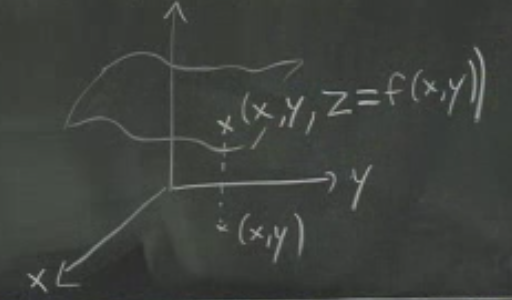
\includegraphics[height=4cm]{8_1.png}

$x,y$ degerlerine tekabul eden $f(x,y)$'yi, z ekseni uzerindeki yukseklik
olarak kabul ederiz, ve oraya bir nokta koyariz. Tum $x,y$'ler icin bu
yapilirsa bir yuzey ortaya cikar. Dikkat 3 boyutlu bir sekil gorulecektir,
fakat ici dolu degildir, fonksiyon sadece yuzeydedir. 

Ornek

\[ f(x,y) = -y \]

2 degiskenli de olsa illa her iki degisken fonksiyonda kullanilmali diye
bir sart yok. Bu formul bir duzlem tanimlar. 

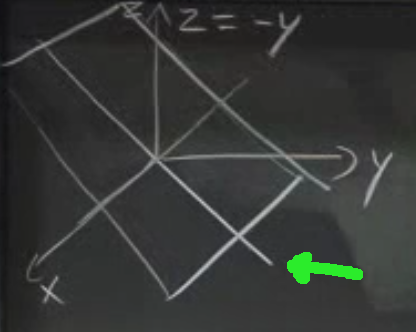
\includegraphics[height=4cm]{8_2.png}

Hoca cizmek icin once yesil okun gosterdigi cizgiden basladi, ki bu cizgi
$z=-y$, -1 egimi olan bir cizgi. $x$ tanimli olmadigina gore bu cizgi her
$x$ icin gecerli olmali, ve ustteki duzlem ortaya cikiyor. x-ekseni bu
duzlemin icinden geciyor. 

Ornek 

\[ f(x,y) = 1-x^2-y^2 \]

Grafigi anlamak icin $yz$ duzleminde neler oluyor onu anlamaya
ugrasalim. Sadece $yz$ duzlemine bakmak demek, $x=0$ kabul etmek demektir,
o zaman geri kalanlar 

\[ z = 1-y^2 \]

bir parabolu tanimlar. 

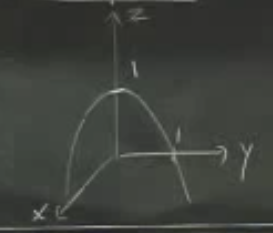
\includegraphics[height=4cm]{8_3.png}

Peki $xz$ duzleminde neler olur?

\[ z = 1- x^2 \]

yine asagi donuk bir parabol. 

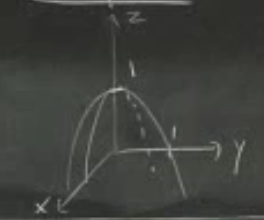
\includegraphics[height=4cm]{8_4.png}

$xy$ duzlemiyle nerede kesisim olur? $z=0$ ise, 

\[ 1-x^2-y^2 = 0 \]

\[ x^2 + y^2 = 1 \]

Bu birim yaricapi olan bir cemberdir (unit circle). 

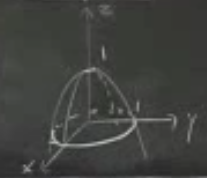
\includegraphics[height=4cm]{8_5.png}

Ilginc bir diger fonksiyon

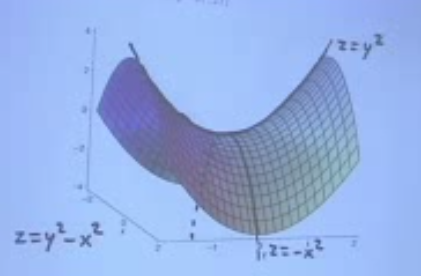
\includegraphics[height=4cm]{8_6.png}

Bir at egerine (saddle) benziyor, $yz$ duzleminden bakilinca yukari giden
bir parabol $z=y^2$, ama $xz$ duzleminde asagi donuk bir parabol, $z=-x^2$. 

Kontur Grafikleri (Contour Plot)

2 degiskenli fonksiyonlari cizmenin bir diger yolu onun konturlarini
cizmektir. Konturlar yeryuzunu resmetmek icin kullanilan haritalara
benzerler, 3 boyutlu sekillerin yassilastirilarak, sadece ustten
gorunuslerini gosteren grafikleme sekilleridirler. 

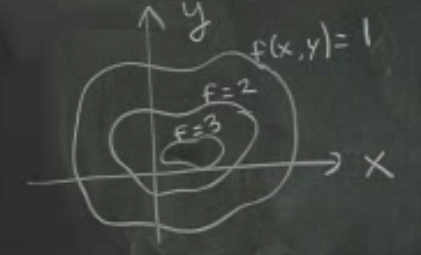
\includegraphics[height=4cm]{8_7.png}

Bir kontur grafigi uzerindeki cizgilerin her biri, bir yukseklige
(elevation) tekabul eder. Mesela $f(x,y)=1$ esitligi icin olan tum $x,y$
noktalari ustte en distaki kapali egridir, $f=2$, $f=3$, vs ayni sekilde. 3
boyutlu ``normal'' bir grafikte yukseklik olarak (3. boyut) temsil edilen
degerler yassilastirilarak onlarin ustten gorunusu resmedilir. Ayrica bir
$z$ ``sabitlenerek'' ona tekabul eden $x,y$ grafiklenir (bu sabit degerler
cogunlukla duzenli araliklarla olacak sekilde secilir, 1,2,3,4,vs gibi), 3
boyutlu bir resimde tum $z$ degerleri grafiklenir. Farkliliklar
bunlardir. Konturlar kullanarak 3 boyutlu bir fonksiyonu iki boyutta kismen
temsil edebilmis oluruz. 3 boyutlu fonksiyon ve $z=1$ anindaki bir kesit
ornegi alttadir. 

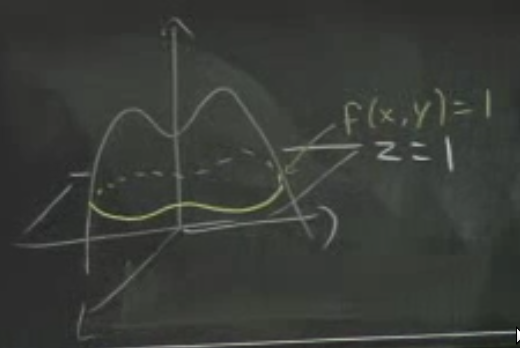
\includegraphics[height=4cm]{8_8.png}

Bu teknige ``seviye egrileri (level curve)'' ismi de verilir. $z=1$
seviyesinde kesit yapilinca o kesit uzerinde bir egri olusur, diger
seviyelerde de kesitler yapilabilir, vs. 

Bir topografik harita da aslinda bir kontur grafigidir. Mesela alttaki
harita ABD Jeolojik Olcumler (US Geological Survey) haritalarindan biri

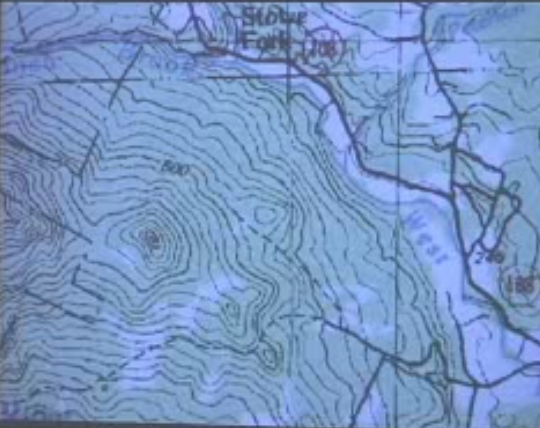
\includegraphics[height=4cm]{8_9.png}

Mesela 500 yazan bir cizgi var, bu yuksekligi gosteriyor. Eger o
yukseklikte kalmak istersek, hep o cizgi uzerinde yuruyebilirdik, ve hic
yukari ya da asagi gitmemis olurduk. Eger cizgiler arasinda gidip gelirsek,
o zaman yukseklik degisimi yapmis olurduk. 

Tabii kontur grafiklerinin illa bir cografi yuksekligi temsil etmesi
gerekmez. Mesela alttaki grafik ABD haritasinda herhangi kac derece
sicaklik oldugunu bolgesel olarak gosteriyor. 

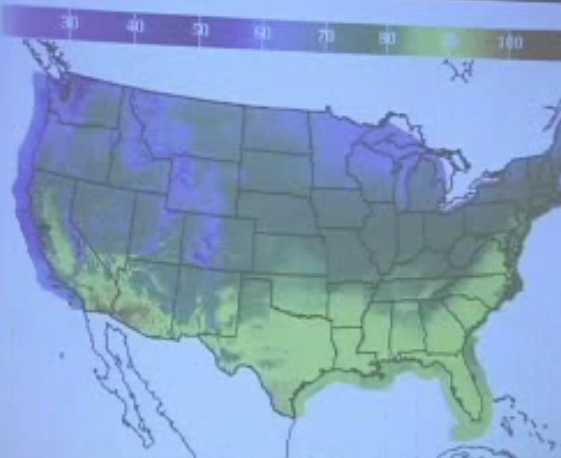
\includegraphics[height=4cm]{8_10.png}

Renkler belli sicakliklari temsil ediyorlar, ve renkler arasinda bazi
sinirlar var. Bu grafik te bir kontur grafigidir. 

Ornek

\[ f(x,y) = -y \]

Konturlar neye benzer? 

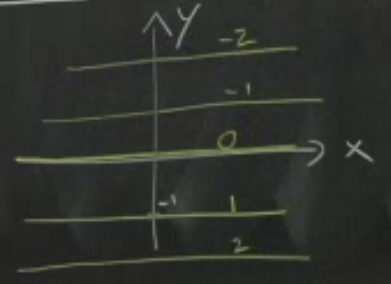
\includegraphics[height=4cm]{8_11.png}

Konturlar degisik yukseklikleri temsil ediyor, ve ustteki resim icin de bu
gecerli. Bu grafigin 3D hali icinde yesil ok olan en ustten 2. grafik. O
grafikte bir duz yokus var, iste ustteki cizgiler, bu yokustaki yukseklik
farkinda tekabul ediyorlar. 

Ornek

\[ f(x,y) = 1-x^2-y^2 \]

Bu fonksiyon sifir ise birim cember olur dedik, yani

\[ x^2+y^2=1 \]

Eger $f=1$ ise

\[ x^2+y^2=0 \]

Eger $f=-1$ ise

\[ x^2+y^2=2 \]

Eger $f=-2$ ise

\[ x^2+y^2=3 \]

Grafik soyle

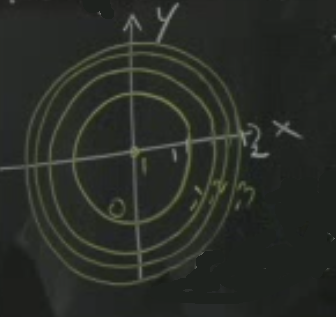
\includegraphics[height=4cm]{8_12.png}

Seviye egrilerinin disa dogru nasil daha s�kla�t���na dikkat cekmek
isterim. Bu demektir ki disa dogru gittikce yukseklik artisi daha dik hale
geliyor, cunku (yukari dogru) ayni birim mesafeyi almak icin gittikce daha
az mesafe katetmek gerekiyor. Orta kisim neredeyse dumduz. 

Ornek

At egrisi grafiginin konturlari

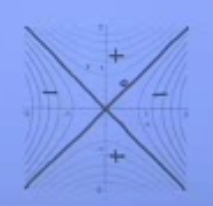
\includegraphics[height=4cm]{8_13.png}

Kontur grafikleri bize $x,y$ degisirken neler oldugunu soyler. Mesela
degerler azaliyor mu, cogaliyor mu? Bu tur bir sorunun cevabini kontur
grafigi hizli bir sekilde saglayabilir. 

Mesela su grafige bakalim

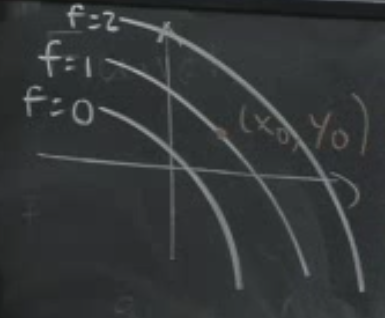
\includegraphics[height=4cm]{8_14.png}

Eger $x$ $\uparrow$, $f(x,y)$ $\uparrow$

Eger $x$ $\downarrow$, $f(x,y)$ $\downarrow$

Eger $y$ $\uparrow$, $f(x,y)$ $\uparrow$

Eger $y$ $\downarrow$, $f(x,y)$ $\downarrow$

Bu tur nicelik analiz kontur grafiklerinin cizgilerine bakarak hemen
yapilabilir. Ama belki de ben daha detayli bir analiz istiyorum, mesela
bir degiskeneki bir degisimin $f(x,y)$'daki degisimi ne kadar etkiledigini
detayli sekilde gormek istiyorum.

Degisim oranlarinin hesabi turevlerle yapilir. 

Kismi Turevler (Partial Derivatives)

Tek degiskenli fonksiyonlar, mesela $f(x)$ gibi, o zaman $f(x)$'in turevi
bir limit olarak tanimlidir

\[ f'(x) = \frac{df}{dx}  = 
\lim_{\Delta x \to 0} \frac{f(x+\Delta x) - f(x)}{\Delta x}
\]

Grafiksel olarak

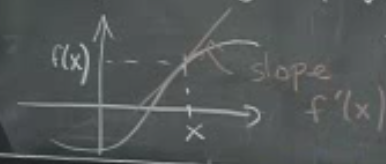
\includegraphics[height=3cm]{8_15.png}

$x$ noktasindaki egim (slope) $f'(x)$'e esittir. 

Yaklasiksallik Formulu

\[ f(x) \approx f(x_0) + f'(x_0)(x-x_0) \]

Bu formule daha fazla terim eklesek, ortaya Taylor Formulu cikardi. 

Benzer seyleri 2 degiskenli fonksiyonlar icin nasil yapardik?

Buradaki problem iki degiskenin ikisinin birden degisebilecegi. Bu sebeple
bize birden fazla turev sekli gerekiyor. 

Notasyon

Parcali turev kivrik bir ``d'' sembolunu andirir

\[ \frac{\partial f}{\partial x} \]

Bu ibare ``sadece $x$ degisiyor, digerleri degismiyor'' demek. O yuzden bu
klasik bir turev degil, kismi bir turev. Tamami

\[ \frac{\partial f}{\partial x}(x_0,y_0) = 
\lim_{\Delta x \to 0} \frac{f(x_o+\Delta x, y_o) - f(x_0,y_0)}{\Delta x}
 \]

Gordugumuz gibi $y$ uzerinde hicbir degisiklik yapmiyorum. Sadece $x$'i
degistirip, bu degisimin fonksiyonun tamami uzerindeki oranini (rate of
change) hesapliyorum. Ayni sekilde

\[ \frac{\partial f}{\partial y}(x_0,y_0) = 
\lim_{\Delta y \to 0} \frac{f(x_o, y_o+\Delta y) - f(x_0,y_0)}{\Delta y}
 \]

Geometriksel olarak

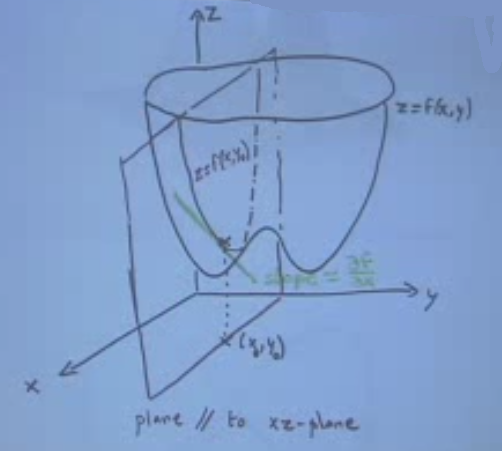
\includegraphics[height=6cm]{8_16.png}

Ustteki $\partial f / \partial x$. Bir $x_0,y_0$ noktasina bakiyorum, sonra
$y$'nin hic degismemesi durumunun ortaya cikaracagi bir duzlem hayal
ediyorum. Sonra bu duzlemin $f$'ten aldigi ``kesiti'' dusunuyorum, iste bu
yansima bir yeni fonksiyon yaratiyor, ve bu fonksiyona $x_0,y_0$ noktasinda
teget gecen cizginin egimi (slope),  $\partial f / \partial x$. 

Peki bu hesap nasil yapilir? Bu arada notasyon olarak 

\[ \frac{\partial f}{\partial x} = f_x \]

ayni seyler. Soldaki fizik notasyonu, sagdaki uygulamali matematik
notasyonu [burada hoca uygulamali matematik, zaten notasyonu degistirilmis
fizik sadece diye espri yapiyor]. Her neyse, hesap icin $y$ sabit tutulur,
$x$ degisken kalir. 

Ornek

\[ f(x,y) = x^3y  + y^2 \]

\[ \frac{\partial f}{\partial x} = 3x^2y + 0\]

\[ \frac{\partial f}{\partial y} = x^3 + 2y\]

Ornekler 

Python Matplotlib ile kesit seviyeleri cizmek icin ornek bir program

\begin{minted}{python}
x=linspace(-3,3,40)
y=linspace(-3,3,40)
x,y=meshgrid(x,y)
z=sqrt(x**2+y**2)
z=x**2+y**2
cs=contour(x,y,z,15)
grid(True)
axis('scaled')
xlabel('x-axis')
ylabel('y-axis')
clabel(cs,inline=1,fontsize=9)
plt.savefig('levels.png')
\end{minted}

$x^2+y^2$ fonksiyonun grafigi alttadir. 

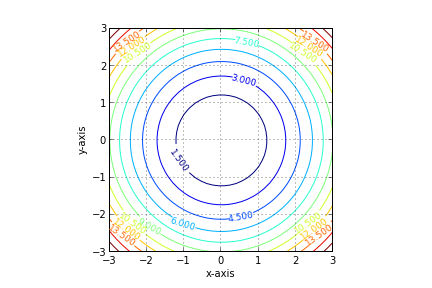
\includegraphics[height=8cm]{levels.png}


Soru 2D-5

$T = x^2 + 2y^2 + 2z^2$ fonksiyonu her $x,y,z$ noktasindaki sicakligi rapor
ediyor. 

a) Bu fonksiyonun isosicaklik (isotherms) fonksiyonu hangi sekle benzer? 

Cevap 

Isosicaklik $T$ fonksiyonun bir sabite esitlendiginde elde edilen
fonksiyondur, o ``sey'' ne ise, o cisim yuzeyinde sicaklik hic
degismeyecektir. 

Bu cisim bir ellipsoid, bir ellipsoid bir yumurtaya benzeyen, bir elips'in
alip bir nevi cevrilerek elde edilen bir sekildir. Peki seklin ellipsoid
oldugunu nereden biliyoruz? Cunku ellipsoid formulu

\[ \frac{x^2}{a^2} +  \frac{y^2}{b^2} + \frac{z^2}{c^2}  = 1  \]

seklinde, ve $x^2 + 2y^2 + 2z^2 = c$ formulunu ustteki forma cevirmek
mumkun. Iki tarafi $c$'ye boleriz,

\[ \frac{x^2}{c} +  \frac{2y^2}{c} + \frac{2z^2}{c}  = 1  \]

Boylece $1/a^2 = 1/c$ olur, vs.. 

Peki bir ellipsoid'i nasil grafikleriz? Bu noktada sorunun istediginden
daha ileri gidiyoruz. 

Grafiklerken, mesela $x^2 + 2y^2 + 2z^2 = 10$ icin diyelim, ilk aklimiza
gelebilecek fikir formulu tekrar organize ederek $z$'yi yanliz birakmak, ve
$x,y$ kombinasyonlarini bu fonksiyona gecerek sonuclari grafiklemek. 

Buradaki problem $z$ formulu ortaya bir karekok cikartacak, ve bu karekok
sonucu hem eksi, hem arti olabilir. Daha iyi bir yontem, kutupsal forma
gecmek, boylece hep arti olacak vektor buyuklugu ve acilar uzerinden bir
cizim yapmak [1]. Su formule tekrar bakarsak

\[ \underbrace{\frac{x^2}{a^2} +  \frac{y^2}{b^2}}_{w^2}
 + \frac{z^2}{c^2}  = 1  \]

bunu

\[ w^2 + \frac{z^2}{c^2}  = 1  \]

olarak gorelim, burada karelerinin toplami '1' olan bir sey var. 

Bu ``seyler'' $\cos$ ve $\sin$ olabilirler, cunku $\cos$ ve $\sin$ karelerinin
toplami 1 degerini verir.

Eger

\[ w = \sin \phi \]

\[ \frac{z}{c} = \cos \phi \]

dersek, karelerin toplami ustteki gibi 1 olur. 

Simdi $w$'nin detayina inelim

\[ w^2 = \sin^2\phi = \frac{x^2}{a^2} +  \frac{y^2}{b^2}  \]

Esitligin en sagina bakarsak, yine kareler toplami goruyoruz. Ama bu sefer
karelerin toplami 1 degil, $\sin^2\phi$ vermis. Problem degil, karelerin
icine bir $\sin \phi$ biz sokarsak, o zaman sonucta istedigimiz bir
ekstra $\sin^2\phi$ kendiliginden gelecek. 

\[ \frac{x}{a} = \sin\phi \cos \theta  \]

\[ \frac{y}{b} = \sin\phi \sin\theta  \]

O zaman

\[ x = a \sin\phi \sin \theta  \]

\[ y = b \sin\phi \cos \theta  \]

\[ z = c \cos \phi \]

O zaman grafiklemeyi $\phi$, $\theta$ acilarinin $0..\pi$ arasindaki degerlerinin 
kombinasyonlarini kullanarak rahatca yapabiliriz. Alttaki kodda
\verb!linspace! ile bu ayriksal degerleri bulunuyor, \verb!outer! ile
onlarin her turlu kombinasyonla carpimi aliniyor. 

Not: $w$ ile $z/c$'nin aldigi $\cos, \sin$ degerleri ters sekilde de olabilir,
sonuc farketmiyor, yine ellipsoid grafikleniyor. 

\begin{minted}{python}
from __future__ import division

from mpl_toolkits.mplot3d import Axes3D

fig = plt.figure(figsize=plt.figaspect(1))  # Square figure
ax = fig.add_subplot(111, projection='3d')

# Katsayilar a0/c x**2 + a1/c y**2 + a2/c z**2 = 1 
coefs = (1, 4, 10)  

# Katsayilara tekabul eden caplar
rx, ry, rz = [1/np.sqrt(coef) for coef in coefs]

u = np.linspace(0, 2 * np.pi, 100)
v = np.linspace(0, np.pi, 100)

x = rx * np.outer(np.cos(u), np.sin(v))
y = ry * np.outer(np.sin(u), np.sin(v))
z = rz * np.outer(np.ones_like(u), np.cos(v))

ax.plot_surface(x, y, z,  rstride=4, cstride=4, color='b')

max_radius = max(rx, ry, rz)
ax.set_xlim(-max_radius, max_radius)
ax.set_ylim(-max_radius, max_radius)
ax.set_zlim(-max_radius, max_radius)

plt.savefig('ellipsoid.png')
\end{minted}

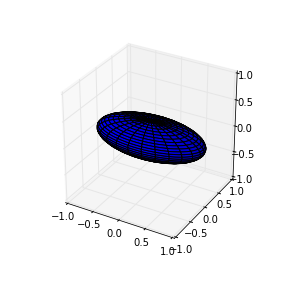
\includegraphics[height=8cm]{ellipsoid.png}

[1] Thomas Calculus, 11. Baski


\end{document}
